\documentclass[tikz,border=2pt]{standalone}
\usepackage{amsmath,amssymb}
\usepackage{tikz}
\usetikzlibrary{arrows.meta}

\begin{document}
% Minimising f (bowl with level circles) subject to g(x) >= b: the feasible region lies above
% the line, the unconstrained minimum is infeasible, and at the constrained minimum the
% gradient of f points INTO the feasible side, parallel to the constraint gradient.
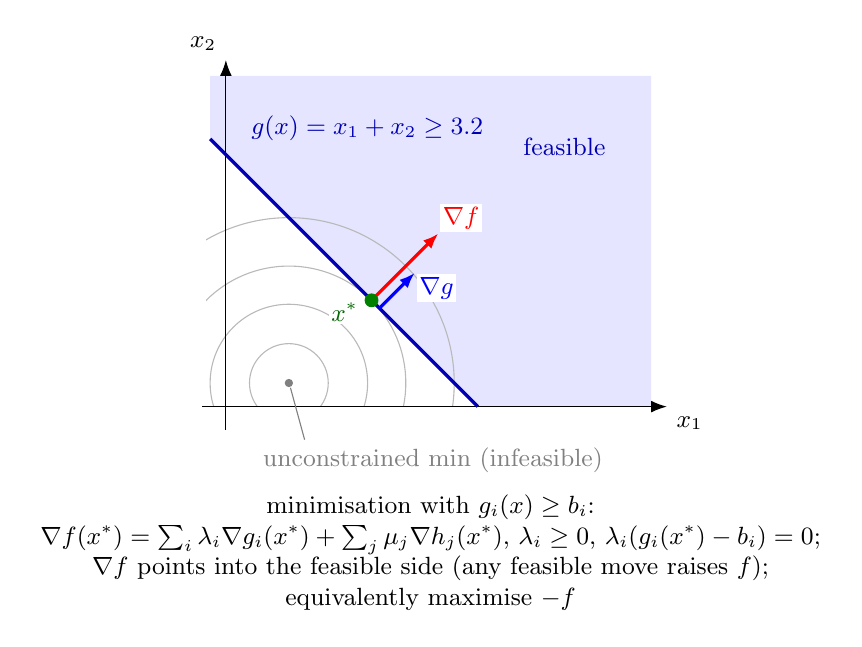
\begin{tikzpicture}[every node/.style={font=\small}, >={Latex[length=2mm]}, lab/.style={font=\small, fill=white, inner sep=1pt}]
	\fill[blue!10] (-0.2,3.4) -- (3.2,0) -- (5.4,0) -- (5.4,4.2) -- (-0.2,4.2) -- cycle;
	\begin{scope}
		\clip (-0.25,0) rectangle (5.4,4.2);
		\foreach \r in {0.5,1.0,1.485,2.1} {\draw[gray!55] (0.8,0.3) circle (\r);}
	\end{scope}
	\draw[->] (-0.3,0) -- (5.6,0) node[below right] {$x_1$};
	\draw[->] (0,-0.3) -- (0,4.4) node[above left] {$x_2$};
	\draw[blue!70!black, very thick] (3.2,0) -- (-0.2,3.4);
	\node[blue!70!black, anchor=south west, font=\small] at (0.2,3.25) {$g(x)=x_1+x_2\ge3.2$};
	\node[blue!70!black, font=\small] at (4.3,3.3) {feasible};
	\fill[gray] (0.8,0.3) circle (1.5pt);
	\draw[gray, thin] (0.82,0.24) -- (1.0,-0.42);
	\node[gray, font=\small, anchor=north west] at (0.35,-0.4) {unconstrained min (infeasible)};
	\draw[->, red, very thick] (1.85,1.35) -- (2.7,2.2) node[above right, lab] {$\nabla f$};
	\draw[->, blue, very thick] (1.95,1.25) -- (2.4,1.7) node[below right, lab] {$\nabla g$};
	\fill[green!50!black] (1.85,1.35) circle (2.5pt);
	\node[green!40!black, anchor=east, lab] at (1.72,1.2) {$x^\ast$};
	\node[anchor=north, align=flush center, text width=10cm] at (2.6,-1.0) {minimisation with $g_i(x)\ge b_i$: $\nabla f(x^\ast)=\sum_i\lambda_i\nabla g_i(x^\ast)+\sum_j\mu_j\nabla h_j(x^\ast)$, $\lambda_i\ge0$, $\lambda_i(g_i(x^\ast)-b_i)=0$; $\nabla f$ points into the feasible side (any feasible move raises $f$); equivalently maximise $-f$};
\end{tikzpicture}
\end{document}
